\documentclass[10pt]{article}
\usepackage[utf8]{inputenc}
\usepackage[includehead, headheight=10mm, margin=15mm ]{geometry}
\usepackage{amsmath}
\usepackage{amsthm}
\usepackage{amsfonts}
\usepackage{xcolor}
\usepackage{graphicx}
\usepackage{titling}
\usepackage{fancyhdr}
\usepackage{listings}

\title{APPM 4600 Homework 4}
\author{Edward Wawrzynek}
\date{27 September 2024}

\newcommand*{\dif}{\mathop{}\!\mathrm{d}}

\makeatletter
\def\@maketitle{%
  \newpage
  \null
  \vskip 1em%
  \begin{center}%
  \let \footnote \thanks
    {\LARGE \@title \par}%
    \vskip 1em%
    {\normalfont \@date}
  \end{center}%
  \par
  \vskip 1em}
\makeatother

\begin{document}

\pagestyle{fancy}
    \fancyhf{} % clear all header and footer fields
    \fancyhead[L]{\thetitle}
    \fancyhead[R]{\theauthor}

\makeatletter
\begin{center}
    {\Large \@title}
    \vskip 1mm
    {\normalfont \@date}
    \vskip 1em
\end{center}
\makeatother

\begin{enumerate}
  \item The code used in this question is listed at the end of the question. \begin{enumerate}
    \item We are interested in the depth at which the temperature reaches 0 after 60 days. If \(T(x,t)\) is the temperature at depth \(x\) and time \(t\), we are interested in the root of the function \begin{align*}
        f(x) = T(x,t=60\;\mathrm{days}) = (T_i - T_s)\mathrm{erf}\left( \frac{x}{2\sqrt{\alpha (60\;\mathrm{days})}} \right) + T_s.
    \end{align*} We have derivative \begin{align*}
        f'(x) = (T_i-T_s) \frac{e^{-\frac{x^2}{4\alpha(60\;\mathrm{days})}}}{\sqrt{\pi}\sqrt{\alpha(60\;\mathrm{days})}}.
    \end{align*}
    This function is plotted over \(x \in [0, 1]\) below.

    \begin{center}
      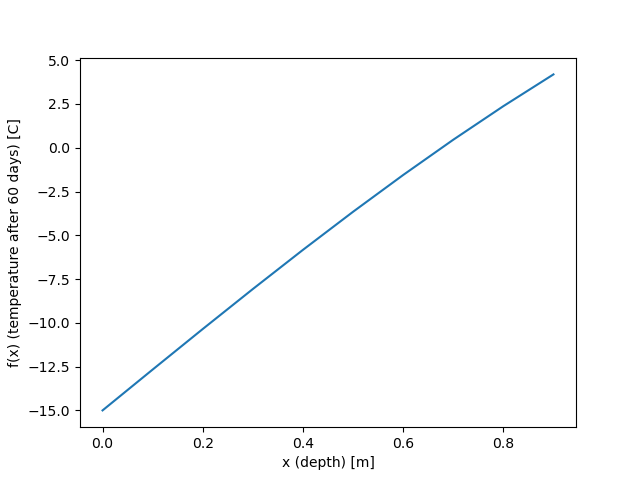
\includegraphics[width=0.5\textwidth]{hw4_1.png}
    \end{center}

    \item Bisection over \([0,1]\) yields an approximate root of \begin{align*}
        x^* \approx0.6769618544819309\;\mathrm{m}.
    \end{align*}

    \item Newton's Method starting at \(x_0 = 0.01\) yields an approximate root \begin{align*}
        x^* \approx 0.6769618544819365.
    \end{align*} As expected, this is within \(\epsilon\) of the root we found via bisection.

    If we start at \(x_0 = \bar{x}\), it is possible that the function's derivative will evaluate to zero and Newton will be unable to find the root. If we evaluate with \(x_0 = 1\), Newton successfully finds the same root as above. 

    {\small \lstinputlisting[language=Python]{hw4_1.py}}
  \end{enumerate}

  \newpage
  \item \begin{enumerate}
    \item A function \(f(x)\) has a root \(\alpha\) of multiplicity \(m\) if there exists some \(q(x)\) such that \begin{align*}
      f(x) = (x-\alpha)^mq(x),
    \end{align*} where \(\lim_{x\to\alpha}q(x) \neq 0\).

    \vspace{0.5cm}

    We have that \(f(x)\) has a root \(\alpha \) of multiplicity \(m\) iff \begin{align*}
        0 = f(\alpha ) = f'(\alpha ) = \dots = f^{(m-1)}(\alpha )\;\;\mathrm{and}\;\;f^{(m)}(\alpha) \neq 0.
    \end{align*}

    \item Let the root \(\alpha\) have multiplicity \(m \geq 2\). The Newton step is \begin{align*}
        x_{n+1} = g(x_n) = x_n - \frac{f(x_n)}{f'(x_n)}.
    \end{align*} Notice that \begin{align*}
        g'(x) = 1 - \frac{f'(x)^2 - f(x)f''(x)}{f'(x)^2} = \frac{f(x)f''(x)}{f'(x)^2}.
    \end{align*} Since the root has multiplicity \(m\), we must have \(f(x) = (x-\alpha)^mq(x)\), where \(q(\alpha ) \neq 0\), so \begin{align*}
        g'(x) &= \frac{(x-\alpha)^mq(x)( (x-\alpha )^mq''(x) + 2m(x-\alpha )^{m-1}q'(x) + m(m-1)(x-\alpha)^{m-2}q(x) )}{(m(x-\alpha )^{m-1}q(x) + (x-\alpha )^mq'(x))^2} \\
        &= \frac{(x-\alpha)^mq(x)( (x-\alpha )^mq''(x) + 2m(x-\alpha )^{m-1}q'(x) + m(m-1)(x-\alpha)^{m-2}q(x) )}{(x-\alpha)^{2m-2} (mq(x) + (x-\alpha )q'(x))^2} \\
        &= \frac{q(x)( (x-\alpha )^2q''(x) + 2m(x-\alpha )q'(x) + m(m-1)q(x) )}{ (mq(x) + (x-\alpha )q'(x))^2}
    \end{align*} Near \(x=\alpha\), we have \(q(x) \neq 0\) and therefore \begin{align*}
        g'(x) &\approx \frac{q(\alpha)( (x-\alpha )^2q''(\alpha) + 2m(x-\alpha )q'(\alpha) + m(m-1)q(\alpha) )}{ (mq(\alpha) + (x-\alpha )q'(\alpha))^2} \\
        &\approx \frac{m(m-1)q(\alpha )^2}{m^2q(\alpha )^2} \\
        &\approx \frac{m(m-1)}{m^2} < 1.
    \end{align*}
    Thus, Newton's method converges in linear order near the root.

    \item The Newton step is \begin{align*}
        x_{n+1} = g(x_n) = x_n - m \frac{f(x_n)}{f'(x_n)}.
    \end{align*} Observe that \begin{align*}
        g'(x) = 1 - m\frac{f'(x)^2 - f(x)f''(x)}{f'(x)^2} = \frac{(1-m)f'(x)^2 + mf(x)f''(x)}{f'(x)^2}.
    \end{align*} As before, we have \(f(x) = (x-\alpha )^mq(x)\), where \(q(\alpha) \neq 0\). After some algebra, we obtain \begin{align*}
      g'(x) = (1-m) (x-a)^{2 m} \left(\frac{m q(x)}{x-a}+q'(x)\right)^2+\frac{m
      q(x) \left(2 m (x-a) q'(x)+(a-x)^2 q''(x)+(m-1) m
      q(x)\right)}{\left((x-a) q'(x)+m q(x)\right)^2}.
    \end{align*} Near \(x = \alpha \), we have \(q(x) \neq \alpha\) and therefore \begin{align*}
      g'(x) &\approx (1-m) (x-a)^{2 m} \left(\frac{m q(\alpha)}{x-a}\right)^2m + \frac{mq(\alpha) \left((m-1) mq(\alpha)\right)}{\left(m q(\alpha)\right)^2} \\
      &\approx (1-m) + \frac{m^2(m-1)q(\alpha)^2}{m^2q(\alpha)^2} \\
      &\approx (1-m) + m-1 \\
      &\approx 0.
    \end{align*} Thus, the modified method converges in second order near the root.

    \item Part (c) provides that the modified Newton iteration can be used to restore quadratic convergence of the method for roots of multiplicity more than 1 if the multiplicity of the root is known.
  \end{enumerate}

  \newpage

  \item Let \(\{x_k\}_{k=1}^\infty\) be a sequence that converges to \(\alpha\) with order \(p\). By definition, \begin{align*}
        \lim _{n \to \infty} \frac{|x_{n+1}-\alpha|}{|x_{n} - \alpha|^p} = \lambda,
    \end{align*} where \(\lambda \neq 0\). We have \begin{align*}
      \ln \left( \lim _{n \to \infty}  \frac{|x_{n+1}-\alpha|}{|x_{n} - \alpha|^p} \right) = \lim _{n \to \infty} \ln \left( \frac{|x_{n+1}-\alpha|}{|x_{n} - \alpha|^p} \right) = \lim _{n \to \infty} \left( \ln \left( |x_{n+1} - \alpha| \right) - p \ln  \left(| x_n - \alpha|  \right) \right) = \ln  \lambda,
    \end{align*} that is, \begin{align*}
      \frac{\ln \left( |x_{n+1} - \alpha| \right) - \ln \lambda }{\ln  \left(| x_n - \alpha|  \right)} \to p,
    \end{align*} i.e. a plot of \(\ln \left( |x_{n+1} - \alpha| \right)\) against \(\ln  \left(| x_n - \alpha|  \right)\) has slope \(p\).
  
  \newpage

  \item The code used in this question is listed below.
  \begin{enumerate}
    \item We consider finding the root of \begin{align*}
        f(x) = e^{3x} - 27x^6 + 27x^4e^x - 9x^2e^{2x}
    \end{align*} over (3, 5). We have derivative \begin{align*}
        f'(x) = 3(e^x-6x)(e^x-3x^2)^2. 
    \end{align*} We find numerically that the approximate root is \begin{align*}
      x \approx 3.7330696105827834,
    \end{align*} which is the root of the second term (\(e^x-3x^2\)) in \(f'(x)\). Thus, this root has multiplicity at least 2 and Newton's method converges in first order. Indeed, numerically calculating the order of convergence yields \(\alpha \approx 1.03\).

    \item We have function \begin{align*}
        g(x) = \frac{f(x)}{f'(x)} = \frac{e^{3x} - 27x^6 + 27x^4e^x - 9x^2e^{2x}}{3(e^x-6x)(e^x-3x^2)^2},
    \end{align*} with derivative \begin{align*}
        g'(x) = \frac{6x^2 + e^x(x^2-4x+2)}{(e^x-6x)^2}.
    \end{align*} We apply Newton's method to \(g(x)\) and get the approximate root \begin{align*}
        x \approx 3.733098888224901,
    \end{align*} which is close to before, as expected. The modified method has effectively reduced the multiplicity of the root by 1, so we expect it to converge quadratically. Indeed, numerically calculating the order of convergence yields \(\alpha \approx 1.93\).

    \item We apply the Newton step \begin{align*}
        x_{n+1} = x_{n} - m\frac{f(x)}{f'(x)},
    \end{align*} where \(m\) is the multiplicity of the root. Here, our root has multiplicity \(m=3\). Applying the modified method yields the approximate root \begin{align*}
        x \approx 3.7330818885939974,
    \end{align*} which is close to before, as expected. We expect the modified method to converge quadratically, which it numerically appears to.

    The modified method from question 2 is a useful method, as it preserves quadratic convergence while only requiring the calculations of \(f(x)\) and \(f'(x)\) (as in the regular Newton method).

    {\small \lstinputlisting[language=Python]{hw4_4.py}}
    \newpage
  \end{enumerate}

  \item The code used in this question is listed below.
  \begin{enumerate}
    \item We have the function \begin{align*}
        f(x) = x^6 -x - 1,
    \end{align*} with derivative \begin{align*}
        f'(x) = 6*x^5 - 1.
    \end{align*} Applying Newton's method with \(x_0 = 2\) yields the root \(x \approx 1.1347241384015194\). The error at each step is shown below in the table. Beyond the first few iterations, each iteration gives about twice as many correct digits as the previous, suggesting quadratic convergence.

    \begin{center}
      \begin{tabular}{c|c}
        $n$ & Absolute Error \\
        \hline 
        1  &  0.8652758615984806 \\
2  &  0.5459041338497894 \\
3  &  0.296014849837543 \\
4  &  0.12024681770791701 \\
5  &  0.026814294371793723 \\
6  &  0.0016291357689859343 \\
7  &  6.389942109663593e-06 \\
8  &  9.870171346904044e-11 \\
9  &  0.0 \\
      \end{tabular}
    \end{center}

    Applying secant method with \(x_0=3\), \(x_1=2\) yields the root \(x \approx 1.1347241384015194\), as before. The error at each step is plotted below. The convergence appears to be superlinear but not quadratic---each iteration gives more than a fixed number of new digits but doesn't double the number.

    \begin{center}
      \begin{tabular}{c|c}
        $n$ & Absolute Error \\
        \hline 
        1  &  0.8652758615984806 \\
2  &  0.13472413840151942 \\
3  &  0.11859510614345492 \\
4  &  0.05585363027511803 \\
5  &  0.01706830745996779 \\
6  &  0.0021925881853863682 \\
7  &  9.266960333342844e-05 \\
8  &  4.924528145267004e-07 \\
9  &  1.1030354407637333e-10 \\
10  &  2.220446049250313e-16 \\
11  &  0.0 \\
      \end{tabular}
    \end{center}

    \item A plot of \(\ln |x_{k+1} - \alpha |\) vs \(\ln |x_k - \alpha |\) is below. As we found in question 3, the slope of this plot is the approximate convergence order of the method. As expected, the plot for Newton has a slope of 2 while the line for secant has a slightly lower slope of 1.569. We showed in class that we expect secant to converge with order \(\phi \approx 1.618\).
    \begin{center}
      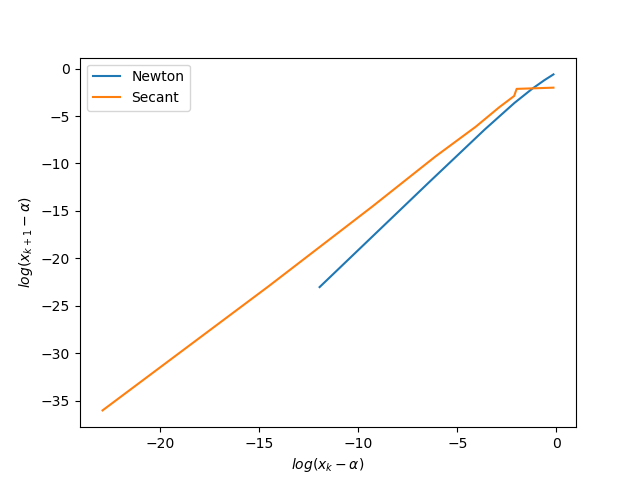
\includegraphics[width=0.5\textwidth]{hw4_5.png}
    \end{center}
  \end{enumerate}

  {\small \lstinputlisting[language=Python]{hw4_5.py}}
\end{enumerate}


\end{document}